%LaTeX reported generated by EES
\documentclass[a4paper,10pt,fleqn]{article}
\mathindent 0.0in
\usepackage[ansinew]{inputenc}
\usepackage{times}
\usepackage{graphicx}
\usepackage{color}
\definecolor{silver}{rgb}{0.75,0.75,0.75}
\definecolor{gray}{rgb}{0.5,0.5,0.5}
\definecolor{aqua}{rgb}{0.5,1,1}
\definecolor{navy}{rgb}{0.0,0.0,0.5}
\definecolor{orange}{rgb}{1.0,0.5,0.0}
\definecolor{teal}{rgb}{0.25,0.5,0.5}
\definecolor{olive}{rgb}{0.5,0.5,0.0}
\definecolor{purple}{rgb}{0.5,0.0,0.5}
\definecolor{brown}{rgb}{0.5,0.25,0.0}
\definecolor{fuchsia}{rgb}{1.0,0.5,1.0}
\definecolor{buff}{rgb}{1.0,0.94,0.80}
\definecolor{lime}{rgb}{0.5,1.0,0.0}
\setlength{\headsep}{-0.6in}
\setlength{\textheight}{9in}
\setlength{\footskip}{1.0 in}
\setlength{\oddsidemargin}{-0.2in}
\setlength{\evensidemargin}{-0.2in}
\setlength{\textwidth}{6.8in}
\usepackage{longtable}
\newcommand{\abs}[1]{\left|#1\right|}
\newcommand{\F}[1]{\mbox{$#1$}}
\newcommand{\K}[1]{\mbox{\sf#1\ \ \mit}}
\newcommand{\KS}[1]{\mbox{\sf\ \ #1\ \ \mit}}
\newcommand{\SC}[1]{\mbox{`#1'}\  }
\newcommand{\V}[1]{\mbox{$ #1 $}}
\newcommand{\I}{\mbox{\hspace{0.20in}}}
\newcommand{\temperature}{\mathrm{T}}
\newcommand{\pressure}{\mathrm{P}}
\newcommand{\volume}{\mathrm{v}}
\newcommand{\density}{\mathrm{\rho}}
\newcommand{\intenergy}{\mathrm{u}}
\newcommand{\enthalpy}{\mathrm{h}}
\newcommand{\entropy}{\mathrm{s}}
\newcommand{\molarmass}{\mathrm{MW}}
\newcommand{\enthalpyfusion}{\mathrm{\Delta h_{fusion}}}
\newcommand{\quality}{\mathrm{x}}
\newcommand{\viscosity}{\mathrm{\mu}}
\newcommand{\conductivity}{\mathrm{k}}
\newcommand{\prandtl}{\mathrm{P_r}}
\newcommand{\cp}{\mathrm{c_p}}
\newcommand{\cv}{\mathrm{c_v}}
\newcommand{\specheat}{\mathrm{c_p}}
\newcommand{\soundspeed}{\mathrm{c}}
\newcommand{\wetbulb}{\mathrm{wb}}
\newcommand{\humrat}{\mathrm{\omega}}
\newcommand{\acentricfactor}{\mathrm{\omega}}
\newcommand{\relhum}{\mathrm{\phi}}
\newcommand{\dewpoint}{\mathrm{DP}}
\newcommand{\volexpcoef}{\mathrm{\beta}}
\newcommand{\compressibilityfactor}{\mathrm{Z}}
\newcommand{\surfacetension}{\mathrm{\gamma}}
\newcommand{\tcrit}{\mathrm{T_{crit}}}
\newcommand{\pcrit}{\mathrm{P_{crit}}}
\newcommand{\vcrit}{\mathrm{v_{crit}}}
\newcommand{\ttriple}{\mathrm{T_{triple}}}
\newcommand{\fugacity}{\mathrm{fugacity}}
\newcommand{\tsat}{\mathrm{T_{sat}}}
\newcommand{\psat}{\mathrm{P_{sat}}}
\newcommand{\eklj}{\mathrm{ek_{LJ}}}
\newcommand{\sigmalj}{\mathrm{\sigma_{LJ}}}
\begin{document}
\begin{center}
\bf \mbox{GLOBAL MODEL - CMI - SD150414 - AUTRE FLUIDE}
\vspace{0.2 in}
\end{center}
\subsection*{Equations}
\begin{equation}
\label{EES Eqn:1}
\K{function} {\Delta P}_{a} \left( \dot {Q},\ \rho_{v},\ \mu_{v},\ A_{v},\ d_{v},\ l_{a},\ h_{lv},\ \V{Re}  \right)  
\end{equation}
\begin{equation}
\I \label{EES Eqn:2}
\K{If} \V{Re}  <2300 \KS{then} 
\end{equation}
\begin{equation}
\I \I \label{EES Eqn:3}
{\Delta P}_{a}=\frac {32\cdot \mu_{v}\cdot \dot {Q}\cdot l_{a}}{ \rho_{v}\cdot A_{v}\cdot h_{lv}\cdot d_{v}^{2} } 
\end{equation}
\begin{equation}
\I \label{EES Eqn:4}
\K{else} 
\end{equation}
\begin{equation}
\I \I \label{EES Eqn:5}
{\Delta P}_{a}= \left( \frac {0.3164}{ Re^{0.25} } \right) \cdot \frac {\dot {Q}^{2}\cdot l_{a}}{ 2\cdot \rho_{v}\cdot A_{v}^{2}\cdot h_{lv}^{2}\cdot d_{v} } 
\end{equation}
\begin{equation}
\I \label{EES Eqn:6}
\K{endif} 
\end{equation}
\begin{equation}
\label{EES Eqn:7}
\K{end} 
\end{equation}
\vspace{0.1 in}
\begin{equation}
\label{EES Eqn:8}
\V{Subprogram}  \V{Caloduc}  \left( PipeMat\$,\ Fluid\$,\ ORCFluid\$,\ d_{i},\ d_{o},\ L_{e},\ L_{c},\ L_{a},\ u_{f},\ \dot {M}_{f},\ \rho_{f},\ T_{in,f},\ P_{f},\ P_{atm},\ T_{ev,wf},\ h_{f,c}:\dot {Q}_{cal},\ \dot {Q}_{limit,ent},\ \dot {Q}_{limit,ebu},\ \dot {Q}_{limit,son},\ T_{we,out},\ T_{sat,e} \right)  
\end{equation}

\vspace{0.10in}
\noindent
\rm Rayons
\begin{equation}
\label{EES Eqn:9}
r_{o}=D_{o}/2 
\end{equation}
\begin{equation}
\label{EES Eqn:10}
r_{i}=D_{i}/2 
\end{equation}

\vspace{0.10in}
\noindent
\bf 1. Evaporateur

\vspace{0.10in}
\noindent
\rm 1.1 Conduction paroi
\begin{equation}
\label{EES Eqn:11}
T_{p,e}=\frac {T_{we,in}+T_{we,out}}{ 2 } 
\end{equation}
\begin{equation}
\label{EES Eqn:12}
\lambda_{e}=k\left( PipeMat\$,\mbox{\ T}=T_{p,e} \right)  
\end{equation}

\vspace{0.10in}
\noindent
\rm 1.2 Evaporation (h$_{e}$)

\vspace{0.10in}
\noindent
\rm Imura correlation
\begin{equation}
\label{EES Eqn:13}
h_{e}=0.32\cdot  \left( \frac {\rho_{l,e}^{0.65}\cdot k_{l,e}^{0.3}\cdot Cp_{l,e}^{0.7}\cdot g\#^{0.2}\cdot q_{e}^{0.4}}{ \rho_{v,e}^{0.25}\cdot h_{lv,e}^{0.4}\cdot \mu_{l,e}^{0.1} } \right) \cdot  \left( P_{sat,e}/P_{atm} \right) ^{0.3} 
\end{equation}
\begin{equation}
\label{EES Eqn:14}
q_{e}=\frac {\dot {Q}_{e}}{ 2\cdot \pi\cdot L_{e}\cdot r_{i} } 
\end{equation}
\begin{equation}
\label{EES Eqn:15}
T_{sat,e}=\tsat \left(\F{Fluid}\$,\mbox{\ P}=P_{sat,e} \right)  
\end{equation}
\begin{equation}
\label{EES Eqn:16}
\rho_{l,e}=\density \left(\F{Fluid}\$,\mbox{\ P}=P_{sat,e},\mbox{\ X}=0 \right)  
\end{equation}
\begin{equation}
\label{EES Eqn:17}
k_{l,e}=\conductivity \left(\F{Fluid}\$,\mbox{\ P}=P_{sat,e},\mbox{\ X}=0 \right)  
\end{equation}
\begin{equation}
\label{EES Eqn:18}
\V{cp} _{l,e}=\cp \left(\F{Fluid}\$,\mbox{\ P}=P_{sat,e},\mbox{\ X}=0 \right)  
\end{equation}
\begin{equation}
\label{EES Eqn:19}
\rho_{v,e}=\density \left(\F{Fluid}\$,\mbox{\ P}=P_{sat,e},\mbox{\ X}=1 \right)  
\end{equation}
\begin{equation}
\label{EES Eqn:20}
h_{lv,e}=\enthalpy \left(\F{Fluid}\$,\mbox{\ P}=P_{sat,e},\mbox{\ X}=1 \right) -\enthalpy \left(\F{Fluid}\$,\mbox{\ P}=P_{sat,e},\mbox{\ X}=0 \right)  
\end{equation}
\begin{equation}
\label{EES Eqn:21}
\mu_{l,e}=\viscosity \left(\F{Fluid}\$,\mbox{\ P}=P_{sat,e},\mbox{\ X}=0 \right)  
\end{equation}
\begin{equation}
\label{EES Eqn:22}
\mu_{v,e}=\viscosity \left(\F{Fluid}\$,\mbox{\ P}=P_{sat,e},\mbox{\ X}=1 \right)  
\end{equation}

\vspace{0.10in}
\noindent
\rm 1.3 Convection et Rayonnement fum�es (h$_{f}$)

\vspace{0.10in}
\noindent
\rm Convection

\vspace{0.10in}
\noindent
\rm Rayonnement id�al
\begin{equation}
\label{EES Eqn:23}
h_{f,r}=sigma\#\cdot \frac { \left( T_{in,f}+273.15 \right) ^{4}- \left( T_{we,out}+273.15 \right) ^{4}}{ T_{in,f}-T_{we,out} } 
\end{equation}

\vspace{0.10in}
\noindent
\rm Somme
\begin{equation}
\label{EES Eqn:24}
h_{f}=h_{f,r}+h_{f,c} 
\end{equation}

\vspace{0.10in}
\noindent
\rm 1.4 Global
\begin{equation}
\label{EES Eqn:25}
\dot {Q}_{e}=\frac {2\cdot \pi\cdot L_{e}\cdot \lambda_{e}}{ \ln{ \left( r_{o}/r_{i} \right) } }\cdot  \left( T_{we,out}-T_{we,in} \right)  
\end{equation}
\begin{equation}
\label{EES Eqn:26}
\dot {Q}_{e}=2\cdot \pi\cdot L_{e}\cdot r_{i}\cdot h_{e}\cdot  \left( T_{we,in}-T_{sat,e} \right)  
\end{equation}
\begin{equation}
\label{EES Eqn:27}
\dot {Q}_{e}=2\cdot \pi\cdot L_{e}\cdot r_{o}\cdot h_{f}\cdot  \left( T_{in,f}-T_{we,out} \right)  
\end{equation}
\begin{equation}
\label{EES Eqn:28}
\dot {M}_{v}=\dot {Q}_{e}/h_{lv,e} 
\end{equation}

\vspace{0.10in}
\noindent
\bf 2 Pertes de charge vapeur

\vspace{0.10in}
\noindent
\rm VDI
\begin{equation}
\label{EES Eqn:29}
A_{v}=0.9\cdot  \left( \pi\cdot r_{i}^{2} \right)  
\end{equation}
\begin{equation}
\label{EES Eqn:30}
A_{v}=\pi\cdot \frac {d_{v}^{2}}{ 4 } 
\end{equation}
\begin{equation}
\label{EES Eqn:31}
\V{Re} _{a}=\frac {\dot {Q}_{e}\cdot d_{v}}{ \mu_{v,c}\cdot A_{v}\cdot h_{lv,c} } 
\end{equation}
\begin{equation}
\label{EES Eqn:32}
{\Delta P}_{a}={\Delta P}_{a} \left( \dot {Q}_{c},\ \rho_{v,c},\ \mu_{v,c},\ A_{v},\ d_{v},\ l_{a},\ h_{lv,c},\ \V{Re} _{a} \right)  
\end{equation}
\begin{equation}
\label{EES Eqn:33}
\V{Re} _{r,c}=\frac {\dot {Q}_{c}\cdot d_{v}/2}{ \mu_{v,c}\cdot A_{c}\cdot h_{lv,c} } 
\end{equation}
\begin{equation}
\label{EES Eqn:34}
A_{c}=2\cdot \pi\cdot L_{c}\cdot r_{i} 
\end{equation}
\begin{equation}
\label{EES Eqn:35}
{\Delta P}_{c}=\frac {{\Delta P}_{a} \left( \dot {Q}_{c},\ \rho_{v,c},\ \mu_{v,c},\ A_{v},\ d_{v},\ l_{c},\ h_{lv,c},\ \V{Re} _{a} \right) }{ 2 } 
\end{equation}
\begin{equation}
\label{EES Eqn:36}
\V{Re} _{r,e}=\frac {\dot {Q}_{e}\cdot d_{v}/2}{ \mu_{v,e}\cdot A_{e}\cdot h_{lv,e} } 
\end{equation}
\begin{equation}
\label{EES Eqn:37}
A_{e}=2\cdot \pi\cdot L_{e}\cdot r_{i} 
\end{equation}
\begin{equation}
\label{EES Eqn:38}
{\Delta P}_{e}=\frac {{\Delta P}_{a} \left( \dot {Q}_{e},\ \rho_{v,e},\ \mu_{v,e},\ A_{v},\ d_{v},\ l_{e},\ h_{lv,e},\ \V{Re} _{a} \right) }{ 2 } 
\end{equation}
\begin{equation}
\label{EES Eqn:39}
{\Delta P}_{ev,cd}=\frac {{\Delta P}_{a}+{\Delta P}_{c}+{\Delta P}_{e}}{ 100000 } 
\end{equation}
\begin{equation}
\label{EES Eqn:40}
P_{sat,c}=P_{sat,e}-{\Delta P}_{ev,cd} 
\end{equation}

\vspace{0.10in}
\noindent
\bf 3. Condenseur

\vspace{0.10in}
\noindent
\rm 3.1 Conduction paroi
\begin{equation}
\label{EES Eqn:41}
T_{p,c}=\frac {T_{wc,in}+T_{wc,out}}{ 2 } 
\end{equation}
\begin{equation}
\label{EES Eqn:42}
\lambda_{c}=k\left( PipeMat\$,\mbox{\ T}=\frac {T_{wc,in}+T_{wc,out}}{ 2 } \right)  
\end{equation}

\vspace{0.10in}
\noindent
\rm 3.2 Condensation

\vspace{0.10in}
\noindent
\rm Rohsenow, Wen and Guo correlation
\begin{equation}
\label{EES Eqn:43}
h_{N}=0.943\cdot k_{l,c}/L_{c}\cdot  \left( \frac {L_{c}^{3}\cdot \rho_{l,c}\cdot  \left( \rho_{l,c}-\rho_{v,c} \right) \cdot g\#}{ \mu_{l,c}\cdot k_{l,c}\cdot  \left( T_{sat,c}-T_{wc,in} \right)  }\cdot  \left( h_{lv,c}+0.68\cdot \V{cp} _{l,c}\cdot  \left( T_{sat,c}-T_{wc,in} \right)  \right)  \right) ^{0.25} 
\end{equation}
\begin{equation}
\label{EES Eqn:44}
P_{sat,c}=\psat \left(\F{Fluid}\$,\mbox{\ T}=T_{sat,c} \right)  
\end{equation}
\begin{equation}
\label{EES Eqn:45}
k_{l,c}=\conductivity \left(\F{Fluid}\$,\mbox{\ P}=P_{sat,c},\mbox{\ X}=0 \right)  
\end{equation}
\begin{equation}
\label{EES Eqn:46}
h_{lv,c}=\enthalpy \left(\F{Fluid}\$,\mbox{\ P}=P_{sat,c},\mbox{\ X}=1 \right) -\enthalpy \left(\F{Fluid}\$,\mbox{\ P}=P_{sat,c},\mbox{\ X}=0 \right)  
\end{equation}
\begin{equation}
\label{EES Eqn:47}
\V{cp} _{l,c}=\cp \left(\F{Fluid}\$,\mbox{\ P}=P_{sat,c},\mbox{\ X}=0 \right)  
\end{equation}
\begin{equation}
\label{EES Eqn:48}
\mu_{l,c}=\viscosity \left(\F{Fluid}\$,\mbox{\ P}=P_{sat,c},\mbox{\ X}=0 \right)  
\end{equation}
\begin{equation}
\label{EES Eqn:49}
\mu_{v,c}=\viscosity \left(\F{Fluid}\$,\mbox{\ P}=P_{sat,c},\mbox{\ X}=1 \right)  
\end{equation}
\begin{equation}
\label{EES Eqn:50}
\rho_{v,c}=\density \left(\F{Fluid}\$,\mbox{\ P}=P_{sat,c},\mbox{\ X}=1 \right)  
\end{equation}
\begin{equation}
\label{EES Eqn:51}
\rho_{l,c}=\density \left(\F{Fluid}\$,\mbox{\ P}=P_{sat,c},\mbox{\ X}=0 \right)  
\end{equation}
\begin{equation}
\label{EES Eqn:52}
h_{c}=1.51\cdot h_{N}\cdot  \left( P_{sat,c}/\pcrit \right) ^{0.15} 
\end{equation}
\begin{equation}
\label{EES Eqn:53}
P_{crit}=\pcrit \left(\F{Water }\right)  
\end{equation}

\vspace{0.10in}
\noindent
\rm 3.3 ORC evaporateur

\vspace{0.10in}
\noindent
\rm Cooper
\begin{equation}
\label{EES Eqn:54}
h_{wf}=55\cdot \V{MM} _{wf}^{-0.5}\cdot q_{c}^{0.67}\cdot p_{r,wf}^{0.12}\cdot  \left( -\log10{ \left( p_{r,wf} \right) } \right) ^{-0.55} 
\end{equation}
\begin{equation}
\label{EES Eqn:55}
p_{r,wf}=\frac {P_{ev,wf}}{ \pcrit \left(\F{ORCFluid}\$ \right)  } 
\end{equation}
\begin{equation}
\label{EES Eqn:56}
\V{MM} _{wf}=\molarmass \left(\F{ORCFluid}\$ \right)  
\end{equation}
\begin{equation}
\label{EES Eqn:57}
P_{ev,wf}=\psat \left(\F{ORCFluid}\$,\mbox{\ T}=T_{ev,wf} \right)  
\end{equation}

\vspace{0.10in}
\noindent
\rm 3.4 Global
\begin{equation}
\label{EES Eqn:58}
\dot {Q}_{c}=\dot {Q}_{e} 
\end{equation}
\begin{equation}
\label{EES Eqn:59}
\dot {Q}_{c}=2\cdot \pi\cdot L_{c}\cdot r_{o}\cdot h_{wf}\cdot  \left( T_{wc,out}-T_{ev,wf} \right)  
\end{equation}
\begin{equation}
\label{EES Eqn:60}
\dot {Q}_{c}=\frac {2\cdot \pi\cdot L_{c}\cdot \lambda_{c}}{ \ln{ \left( r_{o}/r_{i} \right) } }\cdot  \left( T_{wc,in}-T_{wc,out} \right)  
\end{equation}
\begin{equation}
\label{EES Eqn:61}
\dot {Q}_{c}=2\cdot \pi\cdot L_{c}\cdot r_{i}\cdot h_{c}\cdot  \left( T_{sat,c}-T_{wc,in} \right)  
\end{equation}
\begin{equation}
\label{EES Eqn:62}
q_{c}=\frac {\dot {Q}_{c}}{ 2\cdot \pi\cdot L_{c}\cdot r_{i} } 
\end{equation}

\vspace{0.10in}
\noindent
\bf 4 Limites de fonctionnement

\vspace{0.10in}
\noindent
\rm 4.1 Limite d'entrainement

\vspace{0.10in}
\noindent
\rm Habituellement la plus contraignante dans le cas d'un thermosyphon diphasique
\begin{equation}
\label{EES Eqn:63}
\dot {Q}_{limit,ent}=3.2\cdot h_{lv,e}\cdot A_{v}\cdot  \left( \rho_{v,e}^{-0.25}+\rho_{l,e}^{-0.25} \right) ^{-2}\cdot  \left( \sigma_{eau}\cdot g\#\cdot  \left( \rho_{l,e}-\rho_{v,e} \right)  \right) ^{0.25} 
\end{equation}
\begin{equation}
\label{EES Eqn:64}
\sigma_{eau}=\surfacetension \left(\F{Water},\mbox{\ T}=T_{sat,e} \right)  
\end{equation}

\vspace{0.10in}
\noindent
\rm 4.2 Limite d'�bullition
\begin{equation}
\label{EES Eqn:65}
\dot {Q}_{limit,ebu}= \left( \pi\cdot d_{v}\cdot l_{e} \right) \cdot 0.149\cdot \rho_{v,e}\cdot h_{lv,e}\cdot  \left( \frac {\sigma_{eau}\cdot  \left( \rho_{l,e}-\rho_{v,e} \right) \cdot g\#}{ \rho_{v,e}^{2} } \right) ^{0.25} 
\end{equation}

\vspace{0.10in}
\noindent
\rm 4.3 Limite sonique
\begin{equation}
\label{EES Eqn:66}
\dot {Q}_{limit,son}=0.474\cdot A_{v}\cdot h_{lv,e}\cdot  \left( \rho_{v,e}\cdot P_{sat,e}\cdot \rm { \left|100000\ \frac {\rm{Pa}}{\rm{bar}}\right|} \right) ^{0.5} 
\end{equation}
\begin{equation}
\label{EES Eqn:67}
\dot {Q}_{cal}=\dot {Q}_{c} 
\end{equation}
\begin{equation}
\label{EES Eqn:68}
\K{end} 
\end{equation}

\vspace{0.10in}
\noindent
\bf 1. Inputs et param�tres

\vspace{0.10in}
\noindent
\rm 1.1 Caract�ristiques g�om�triques
\begin{equation}
\label{EES Eqn:69}
A_{f}=11.56   \   \left[ \rm m^{2} \right] 
\mbox{\I Aire du conduit de fum�e}
\end{equation}

\vspace{0.10in}
\noindent
\rm 1.2 Mat�riau et fluide
\begin{equation}
\label{EES Eqn:70}
PipeMat\$=\SC{Carbon\_steel} 
\end{equation}
\begin{equation}
\label{EES Eqn:71}
Fluid\$=\SC{Water} 
\end{equation}

\vspace{0.10in}
\noindent
\rm 1.3 Fluides secondaires

\vspace{0.10in}
\noindent
\rm Point de fonctionnement du 11/09/2014 � 15:34:31
\begin{equation}
\label{EES Eqn:72}
\rho_{f,N}=1.242   \   \left[ \rm kg/m^{3} \right] 
\end{equation}
\rm
\begin{equation}
\label{EES Eqn:73}
ORCFluid\$=\SC{n-pentane} 
\end{equation}

\vspace{0.10in}
\noindent
\rm 1.4 Constantes
\begin{equation}
\label{EES Eqn:74}
P_{atm}=1   \   \left[ \rm bar \right] 
\end{equation}
\rm

\vspace{0.10in}
\noindent
\rm 1.5 Echangeur caloduc
\begin{verbatim}
$Constant nbr_cal#=160
\end{verbatim}  \begin{verbatim}
$Constant nbr_rangee#=20
\end{verbatim}  \begin{equation}
\label{EES Eqn:75}
\V{nbr} _{total,cal}=\V{nbr} _{cal\#} 
\end{equation}
\begin{equation}
\label{EES Eqn:76}
\V{nbr} _{rangee,cal}=\V{nbr} _{rangee\#} 
\end{equation}
\begin{equation}
\label{EES Eqn:77}
\V{nbr} _{ligne,cal}=\V{nbr} _{cal\#}/\V{nbr} _{rangee\#} 
\end{equation}
\begin{equation}
\label{EES Eqn:78}
D_{ech}=3.4   \   \left[ \rm m \right] 
\end{equation}
\rm

\vspace{0.10in}
\noindent
\rm 1.6 ORC

\vspace{0.10in}
\noindent
\bf 2 Echange thermique caloduc

\vspace{0.10in}
\noindent
\rm Coefficient de convection moyen
\begin{equation}
\label{EES Eqn:79}
\K{call} \F{External_{Flow,Inline,Bank}}{ \left( \SC{Air},\ T_{in,f},\ T_{out,f},\ T_{we,moy} ,\  1,\ u_{f,1},\ \V{nbr} _{cal\#}/\V{nbr} _{rangee\#},\ D_{o},\ S_{T},\ S_{L}: h_{f,c},\ {\Delta p}_{f},\ \V{Nusselt} _{f},\ \V{Re} _{f} \right) } 
\end{equation}

\vspace{0.10in}
\noindent
\rm Discr�tisation spatiale
\begin{equation}
\label{EES Eqn:80}
T_{f,1}=T_{in,f} 
\end{equation}
\begin{equation}
\label{EES Eqn:81}
\K{duplicate} i=1,\ \V{nbr} _{cal\#}/\V{nbr} _{rangee\#} 
\end{equation}
\begin{equation}
\I \label{EES Eqn:82}
\K{call} \V{Caloduc}  \left( PipeMat\$,\ Fluid\$,\ ORCFluid\$,\ d_{i},\ d_{o},\ L_{e},\ L_{c},\ L_{a},\ u_{f,i},\ \dot {M}_{f},\ \rho_{f,i},\ T_{f,i},\ P_{f},\ P_{atm},\ T_{ev,wf},\ h_{f,c}:\dot {Q}_{cal,i},\ \dot {Q}_{limit,ent,i},\ \dot {Q}_{limit,ebu,i},\ \dot {Q}_{limit,son,i},\ T_{we,out,i},\ T_{sat,e,i} \right)  
\end{equation}
\begin{equation}
\I \label{EES Eqn:83}
\rho_{f,i}=\rho_{f,N}\cdot \frac {273.15}{ T_{f,i}+273.15 } 
\end{equation}
\begin{equation}
\I \label{EES Eqn:84}
u_{f,i}=\frac {\dot {M}_{f}}{ \rho_{f,i}\cdot A_{f} } 
\end{equation}
\begin{equation}
\I \label{EES Eqn:85}
\V{cp} _{f,i}=1300   \   \left[ \rm J/kg^{} \! \cdot \!K \right] 
\end{equation}
\rm
\begin{equation}
\I \label{EES Eqn:86}
T_{f,i+1}=T_{f,i}-\dot {Q}_{cal,i}\cdot \frac {\V{nbr} _{rangee\#}}{ \dot {M}_{f}\cdot cp_{f,i} } 
\end{equation}
\begin{equation}
\label{EES Eqn:87}
\K{end} 
\end{equation}

\vspace{0.10in}
\noindent
\rm Valeurs globales
\begin{equation}
\label{EES Eqn:88}
T_{out,f}=T_{f,nbr,cal\#/nbr,rangee\#+1} 
\end{equation}
\begin{equation}
\label{EES Eqn:89}
T_{we,moy} = \frac {\mbox{Sum}{ \left( T_{we,out,i}\cdot \V{nbr} _{rangee\#},\ i=1,\ \V{nbr} _{cal\#}/\V{nbr} _{rangee\#} \right) }}{ nbr_{cal\#} } 
\end{equation}
\begin{equation}
\label{EES Eqn:90}
\dot {Q}_{total}=\mbox{Sum}{ \left( \dot {Q}_{cal,i}\cdot \V{nbr} _{rangee\#},\ i=1,\ \V{nbr} _{cal\#}/\V{nbr} _{rangee\#} \right) } 
\end{equation}
\begin{equation}
\label{EES Eqn:91}
\dot {Q}_{total,limit,ent}=\mbox{Sum}{ \left( \dot {Q}_{limit,ent,i}\cdot \V{nbr} _{rangee\#},\ i=1,\ \V{nbr} _{cal\#}/\V{nbr} _{rangee\#} \right) } 
\end{equation}
\begin{equation}
\label{EES Eqn:92}
\dot {Q}_{moy}=\dot {Q}_{total}/\V{nbr} _{cal\#} 
\end{equation}
\begin{equation}
\label{EES Eqn:93}
\dot {Q}_{max}=\dot {Q}_{cal,1} 
\end{equation}
\begin{equation}
\label{EES Eqn:94}
\dot {Q}_{min}=\dot {Q}_{cal,nbr,cal\#/nbr,rangee\#} 
\end{equation}
\begin{equation}
\label{EES Eqn:95}
\dot {Q}_{limit,ent,max}=\dot {Q}_{limit,ent,1} 
\end{equation}
\begin{equation}
\label{EES Eqn:96}
\dot {Q}_{limit,ent,min}=\dot {Q}_{limit,ent,nbr,cal\#/nbr,rangee\#} 
\end{equation}
\begin{equation}
\label{EES Eqn:97}
\dot {Q}_{limit,ent,moy}=\dot {Q}_{total,limit,ent}/\V{nbr} _{cal\#} 
\end{equation}

\vspace{0.10in}
\noindent
\bf 3 Performance ORC
\begin{equation}
\label{EES Eqn:98}
\dot {Q}_{ev}=\dot {Q}_{total} 
\end{equation}
\begin{equation}
\label{EES Eqn:99}
P_{ev}=\psat \left(\F{ORCFluid}\$,\mbox{\ T}=T_{ev,wf} \right)  
\end{equation}
\begin{equation}
\label{EES Eqn:100}
P_{cd}=\psat \left(\F{ORCFluid}\$,\mbox{\ T}=T_{cd} \right)  
\end{equation}
\begin{equation}
\label{EES Eqn:101}
h_{in,tur}=\enthalpy \left(\F{ORCFluid}\$,\mbox{\ P}=P_{ev},\mbox{\ X}=1 \right)  
\end{equation}
\begin{equation}
\label{EES Eqn:102}
s_{in,tur}=\entropy \left(\F{ORCFluid}\$,\mbox{\ P}=P_{ev},\mbox{\ X}=1 \right)  
\end{equation}
\begin{equation}
\label{EES Eqn:103}
h_{out,s,tur}=\enthalpy \left(\F{ORCFluid}\$,\mbox{\ s}=s_{in,tur},\mbox{\ P}=P_{cd} \right)  
\end{equation}
\begin{equation}
\label{EES Eqn:104}
w_{s,tur}=h_{in,tur}-h_{out,s,tur} 
\end{equation}
\begin{equation}
\label{EES Eqn:105}
w_{tur}=w_{s,tur}\cdot \epsilon_{s,tur} 
\end{equation}
\begin{equation}
\label{EES Eqn:106}
h_{out,tur}=h_{in,tur}-w_{tur} 
\end{equation}
\begin{equation}
\label{EES Eqn:107}
T_{out,tur}=\temperature \left(\F{ORCFluid}\$,\mbox{\ P}=P_{cd},\mbox{\ h}=h_{out,tur} \right)  
\end{equation}
\begin{equation}
\label{EES Eqn:108}
h_{out,cd}=\enthalpy \left(\F{ORCFluid}\$,\mbox{\ P}=P_{cd},\mbox{\ X}=0 \right)  
\end{equation}
\begin{equation}
\label{EES Eqn:109}
s_{out,cd}=\entropy \left(\F{ORCFluid}\$,\mbox{\ P}=P_{cd},\mbox{\ X}=0 \right)  
\end{equation}
\begin{equation}
\label{EES Eqn:110}
h_{out,s,pp}=\enthalpy \left(\F{ORCFluid}\$,\mbox{\ P}=P_{ev},\mbox{\ s}=s_{out,cd} \right)  
\end{equation}
\begin{equation}
\label{EES Eqn:111}
w_{s,pp}=h_{out,s,pp}-h_{out,cd} 
\end{equation}
\begin{equation}
\label{EES Eqn:112}
w_{pp}=w_{s,pp}/\epsilon_{s,pp} 
\end{equation}
\begin{equation}
\label{EES Eqn:113}
h_{out,pp}=h_{out,cd}+w_{pp} 
\end{equation}
\begin{equation}
\label{EES Eqn:114}
T_{out,pp}=\temperature \left(\F{ORCFluid}\$,\mbox{\ P}=P_{ev},\mbox{\ h}=h_{out,pp} \right)  
\end{equation}
\begin{equation}
\label{EES Eqn:115}
\V{cp} _{out,tur}=\cp \left(\F{ORCFluid}\$,\mbox{\ P}=P_{cd},\mbox{\ h}=h_{out,tur} \right)  
\end{equation}
\begin{equation}
\label{EES Eqn:116}
\V{cp} _{out,pp}=\cp \left(\F{ORCFluid}\$,\mbox{\ P}=P_{ev},\mbox{\ h}=h_{out,pp} \right)  
\end{equation}
\begin{equation}
\label{EES Eqn:117}
\dot {C}_{min}=\V{Min}  \left( \dot {M}_{r}\cdot \V{cp} _{out,tur},\ \dot {M}_{r}\cdot \V{cp} _{out,pp} \right)  
\end{equation}
\begin{equation}
\label{EES Eqn:118}
\dot {Q}_{rec}=\dot {C}_{min}\cdot \epsilon_{rec}\cdot  \left( T_{out,tur}-T_{out,pp} \right)  
\end{equation}
\begin{equation}
\label{EES Eqn:119}
T_{out,rec,fr}=T_{out,pp}+\frac {\dot {Q}_{rec}}{ \dot {M}_{r}\cdot cp_{out,pp} } 
\end{equation}
\begin{equation}
\label{EES Eqn:120}
T_{out,rec,ch}=T_{out,tur}-\frac {\dot {Q}_{rec}}{ \dot {M}_{r}\cdot cp_{out,tur} } 
\end{equation}
\begin{equation}
\label{EES Eqn:121}
\dot {Q}_{total}+\dot {Q}_{rec}=\dot {M}_{r}\cdot  \left( h_{in,tur}-h_{out,pp} \right)  
\end{equation}
\begin{equation}
\label{EES Eqn:122}
\dot {W}_{pp}=\dot {M}_{r}\cdot  \left( h_{out,pp}-h_{out,cd} \right)  
\end{equation}
\begin{equation}
\label{EES Eqn:123}
\dot {W}_{tur}=\dot {M}_{r}\cdot  \left( h_{in,tur}-h_{out,tur} \right)  
\end{equation}
\begin{equation}
\label{EES Eqn:124}
\dot {W}_{net}=\dot {W}_{tur}-\dot {W}_{pp} 
\end{equation}
\begin{equation}
\label{EES Eqn:125}
\eta_{gross,ORC}=\dot {W}_{tur}/\dot {Q}_{total} 
\end{equation}
\begin{equation}
\label{EES Eqn:126}
\eta_{net,ORC}=\dot {W}_{net}/\dot {Q}_{total} 
\end{equation}

\vspace{0.10in}
\noindent
\bf 7 Pertes de charges conduit fum�es
\begin{equation}
\label{EES Eqn:127}
L_{ech}= \left( S_{L}+d_{o} \right) \cdot \V{nbr} _{cal\#}/\V{nbr} _{rangee\#} 
\mbox{\I Encombrement dans le sens de l`�coulement}
\end{equation}
\begin{equation}
\label{EES Eqn:128}
S_{T}=\frac {D_{ech}}{ nbr_{rangee\#}+1 } 
\end{equation}
\begin{equation}
\label{EES Eqn:129}
{\Delta P}=100000\cdot {\Delta P}_{f} 
\end{equation}

\subsection*{Stack effect}
{\centerline{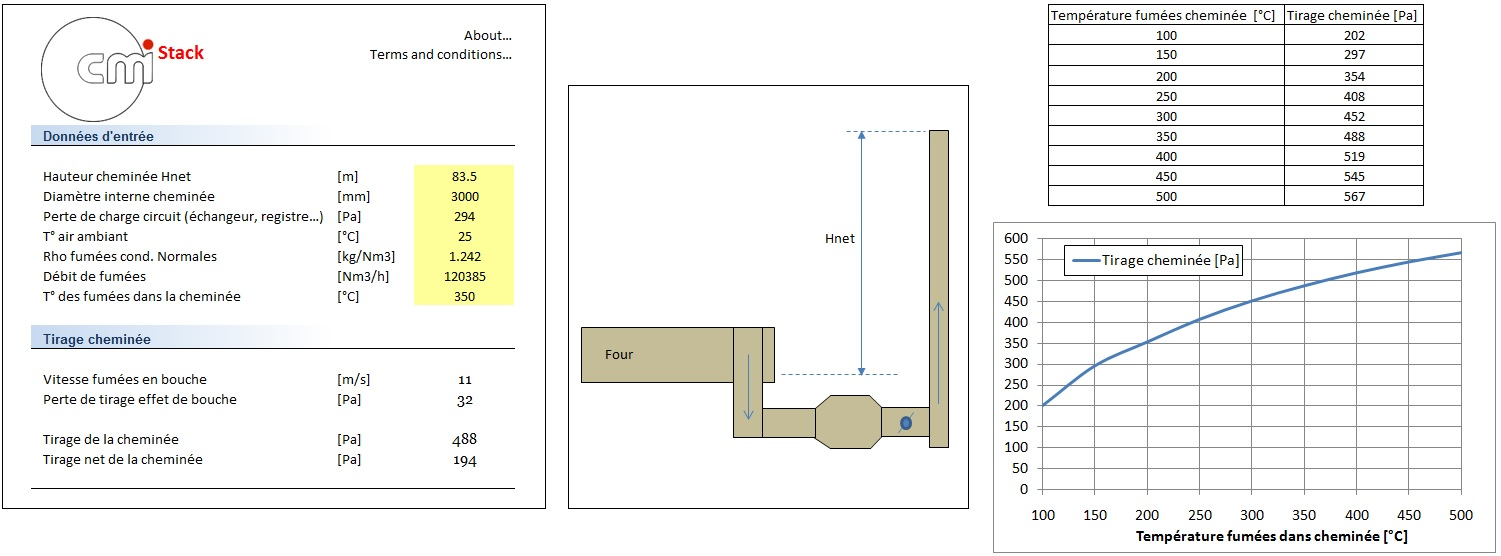
\includegraphics[width=5.0in,keepaspectratio]{Stackeffect.jpg}}
\end{document}

